\documentclass{standalone}

\usepackage{tikz}
\usepackage{tkz-euclide}
\usetikzlibrary{calc}
\usetikzlibrary{positioning}
\usetikzlibrary{arrows.meta}

\usepackage{times}


\begin{document}
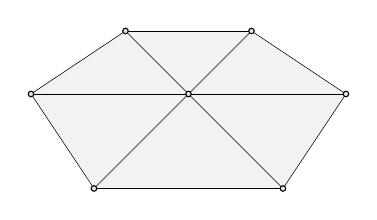
\begin{tikzpicture}[%
  >={Stealth[scale=1.0]},
  scale=2
]

  \tkzDefPoint(0.0, 0.0){x}

  % \tkzDefPointOnCircle[R = center x angle 0 radius 1]\tkzGetPoint{A}
  % \tkzDefPointOnCircle[R = center x angle 60 radius 1]\tkzGetPoint{B}
  % \tkzDefPointOnCircle[R = center x angle 120 radius 1]\tkzGetPoint{C}
  % \tkzDefPointOnCircle[R = center x angle 180 radius 1]\tkzGetPoint{D}
  % \tkzDefPointOnCircle[R = center x angle 240 radius 1]\tkzGetPoint{E}
  % \tkzDefPointOnCircle[R = center x angle 300 radius 1]\tkzGetPoint{F}

  \tkzDefPoint(1.0, 0.0){A}
  \tkzDefPoint(0.4, 0.4){B}
  \tkzDefPoint(-0.4, 0.4){C}
  \tkzDefPoint(-1.0, 0.0){D}
  \tkzDefPoint(-0.6, -0.6){E}
  \tkzDefPoint(0.6, -0.6){F}

  \tkzFillPolygon[color=black!10,opacity=0.5](x,A,B)
  \tkzFillPolygon[color=black!10,opacity=0.5](x,B,C)
  \tkzFillPolygon[color=black!10,opacity=0.5](x,C,D)
  \tkzFillPolygon[color=black!10,opacity=0.5](x,D,E)
  \tkzFillPolygon[color=black!10,opacity=0.5](x,E,F)
  \tkzFillPolygon[color=black!10,opacity=0.5](x,F,A)

  \tkzDefPointOnLine[pos=0.5](x,A)\tkzGetPoint{tmp}
  % \tkzFillCircle[color=black!10,opacity=0.5,R](x)
  % \tkzDrawCircle[black,dashed,fill=black!10,opacity=0.8](x,tmp)

  \tkzDrawSegments(x,A x,B x,C x,D x,E x,F)
  \tkzDrawSegments(A,B B,C C,D D,E E,F F,A)
  \tkzDrawPoints(x,A,B,C,D,E,F)

\end{tikzpicture}
\end{document}
